\section{Datenbus}
Eines der Hauptbestandteile des modularen Eingabesystems ist das Entwerfen und Umsetzen eines leistungsfähigen und flexiblen Datenbusses. Dieser Datenbus dient als Kommunikationsschnittstelle zwischen den verschiedenen Modulen, wie dem Keypad-Modul und dem Audiomodul und ermöglicht dadurch die Datenübertragung zum Hauptmodul. Skalierbarkeit, Zuverlässigkeit und Geschwindigkeit sind die Hauptkriterien des Datenbusses. Ziel ist es, eine einfache Erweiterbarkeit durch Hinzufügen oder Entfernen von Modulen zu ermöglichen, ohne dabei grundlegende Kommunikationsmechanismen zu beeinträchtigen.

\section{Aufbau des Datenbusses}
Der Bus ist nach folgendem Schema aufgebaut:
\begin{itemize}
    \item Start of Frame (SOF) - 2 Bit zum Synchronisieren der Frequenzen; Durch ein HIGH-Value wird der Begin des SOF bekanntgegeben und durch das darauf folgende LOW-Value können die Teilnehmer sich auf die Übertragungsgeschwindigkeit synchronisieren.
    \item Sendeadresse -  3 Bit zum Senden der Adresse; Die Adresse 0x00 ist für neue Teilnehmer reserviert, über diese Adresse findet die Adressvergabe statt. Die Adresse 0x01 ist fest an das Hauptmodul vergeben, alle Teilnehmer wissen das auf dieser Adresse das Hauptmodul liegt. Die Adressen 0x02 bis 0x07 stehen für Teilnehmer zur Verfügung. 3 Bit sind vollkommen aussreichend, da das System als Desktop Erweiterung geplant ist und mehr als 6 Module nicht vorgesehen ist. Sollten in Zukunft mehr Teilnehmer erforderlich sein, lässt sich das im Code leicht anpassen.
    \item Content of Frame (COF) - 3 Bit für Datenlänge in Byte; Das COF enthält die Länge der Übertragenden Daten in Byte. Dies dient dazu, dass die Länge der zu übertragenden Daten dynamisch sein kann (bis zu 8 Byte). Zusätzlich können Teilnehmer welche nicht angesprochen werden festlegen wie lange der Bus belegt ist bevor diese versuchen sollten zu senden.
    \item Daten - 0-8 Byte
    \item ?? (CRC) - X Bit
    \item Enf of Frame (EOF) - 4 Bit Signalende; Vier aufeinanderfolgende LOW-Values geben das Ende der Nachricht an. Ein Teilnehmer der Senden möchte wartet bis er 4 aufeinanderfolgende LOW-Value empfangen hat bevor dieser Sendet.
\end{itemize}

Die folgende Abbildung stellt den Datenbus dar:
\begin{figure}[H]
    \centering    
    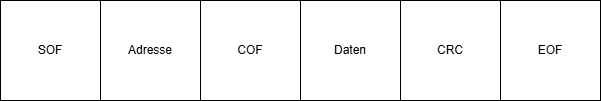
\includegraphics[width=1\textwidth]{Bilder/datenbus.png}
    \caption{Aufbau des Datenbusses}
    \label{Datenbus}
\end{figure}

\subsection{Bitstuffing}
Um Sicherzustellen, dass innerhalb der Datenübertragung keine vier Aufeinanderfolgenden LOW-Value gesendet werden wird das Prinzip des Bitstuffing eingesetzt. Mithilfe einer Laufvariable werden die zu sendenden Bits gezählt und vor dem vierten gleichen Bit wird ein invertiertes Bit gesendet.